% This is "aamas2012 .tex" August 2012 
% This file should be compiled with "aamas2012 .cls" 
% This example file demonstrates the use of the 'aamas2012 .cls'
% LaTeX2e document class file. It is for those submitting
% articles to AAMAS 2012  conference. This file is based on
% the sig-alternate.tex example file.
% The 'sig-alternate.cls' file of ACM will produce a similar-looking,
% albeit, 'tighter' paper resulting in, invariably, fewer pages.
% than the original style ACM style.
%
% ----------------------------------------------------------------------------------------------------------------
% This .tex file (and associated .cls ) produces:
%       1) The Permission Statement
%       2) The Conference (location) Info information
%       3) The Copyright Line with AAMAS data
%       4) NO page numbers
%
% as against the acm_proc_article-sp.cls file which
% DOES NOT produce 1) thru' 3) above.
%
% Using 'aamas2012 .cls' you don't have control
% from within the source .tex file, over both the CopyrightYear
% (defaulted to 200X) and the IFAAMAS Copyright Data
% (defaulted to X-XXXXX-XX-X/XX/XX).
% These information will be overwritten by fixed AAMAS 2012  information
% in the style files - it is NOT as you are used with ACM style files.
%
% ---------------------------------------------------------------------------------------------------------------
% This .tex source is an example which *does* use
% the .bib file (from which the .bbl file % is produced).
% REMEMBER HOWEVER: After having produced the .bbl file,
% and prior to final submission, you *NEED* to 'insert'
% your .bbl file into your source .tex file so as to provide
% ONE 'self-contained' source file.
%

\newtheorem{note}{Note}
\newtheorem{example}{Example}
\newtheorem{definition}{Definition}

% This is the document class for full camera ready papers and extended abstracts repsectively 

\documentclass{aamas2012}

\usepackage{graphicx}
\usepackage{color}
\usepackage{algorithm,algorithmic}
\usepackage{multirow}

\usepackage{module}

\graphicspath{{pictures/}}

% if you are using PDF LaTex and you cannot find a way for producing
% letter, the following explicit settings may help
 
\pdfpagewidth=8.5truein
\pdfpageheight=11truein

\begin{document}

% In the original styles from ACM, you would have needed to
% add meta-info here. This is not necessary for AAMAS 2012  as
% the complete copyright information is generated by the cls-files.


\title{Using Meta-Knowledge on ASP Modules Combination for modular reasoning in Multi-Agent System}

% AUTHORS


% For initial submission, do not give author names, but the
% tracking number, instead, as the review process is blind.

% You need the command \numberofauthors to handle the 'placement
% and alignment' of the authors beneath the title.
%
% For aesthetic reasons, we recommend 'three authors at a time'
% i.e. three 'name/affiliation blocks' be placed beneath the title.
%
% NOTE: You are NOT restricted in how many 'rows' of
% "name/affiliations" may appear. We just ask that you restrict
% the number of 'columns' to three.
%
% Because of the available 'opening page real-estate'
% we ask you to refrain from putting more than six authors
% (two rows with three columns) beneath the article title.
% More than six makes the first-page appear very cluttered indeed.
%
% Use the \alignauthor commands to handle the names
% and affiliations for an 'aesthetic maximum' of six authors.
% Add names, affiliations, addresses for
% the seventh etc. author(s) as the argument for the
% \additionalauthors command.
% These 'additional authors' will be output/set for you
% without further effort on your part as the last section in
% the body of your article BEFORE References or any Appendices.

%\numberofauthors{8} %  in this sample file, there are a *total*
% of EIGHT authors. SIX appear on the 'first-page' (for formatting
% reasons) and the remaining two appear in the \additionalauthors section.
%

\numberofauthors{3}

\author{
% You can go ahead and credit any number of authors here,
% e.g. one 'row of three' or two rows (consisting of one row of three
% and a second row of one, two or three).
%
% The command \alignauthor (no curly braces needed) should
% precede each author name, affiliation/snail-mail address and
% e-mail address. Additionally, tag each line of
% affiliation/address with \affaddr, and tag the
% e-mail address with \email.
% 1st. author
\alignauthor
Tony Ribeiro\\
       \affaddr{National Institute of Informatics}\\
       \affaddr{Tokyo, Japan}\\
       \email{ribeiro@nii.ac.jp}
% 2nd. author
\alignauthor
Katsumi Inoue\\
       \affaddr{National Institute of Informatics}\\
       \affaddr{Tokyo, Japan}\\
       \email{ki@nii.ac.jp}
% 3rd. author
\alignauthor
Gauvain Bourgne\\
       \affaddr{Universit\'e Pierre et Marie Curie}\\
       \affaddr{Paris, France}\\
       \email{bourgne@nii.ac.jp}
}

\maketitle

\begin{abstract}
	In this work, our interest is about multi-agent systems in dynamic environment.
	Here, we focus on one agent regarding knowledge representation and reasoning.
	In such environment, an agent needs to be able to manage his knowledge in a non-monotonic way.
	To reach his goals in a changing context, he have to adapt his beliefs and behaviour regarding the current state of the world.
	Our objective is to define a method which makes easier to design agent knowledge and reasoning in a dynamic context.
	For this purpose, we use the expressibility of answer set programming to propose a method based on ASP modules combinations.
	By using meta-knowledge on these combinations we represent dynamic behaviours and meta-reasoning.
	We also propose a framework and a algorithm to implement and use this method in multi-agent systems.
\end{abstract}

% Note that the category section should be completed after reference to the ACM Computing Classification Scheme available at
% http://www.acm.org/about/class/1998/.

\category{H.4}{Information Systems Applications}{Miscellaneous}

%A category including the fourth, optional field follows...
%\category{D.2.8}{Software Engineering}{Metrics}[complexity measures, performance measures]

%General terms should be selected from the following 16 terms: Algorithms, Management, Measurement, Documentation, Performance, Design, Economics, Reliability, Experimentation, Security, Human Factors, Standardization, Languages, Theory, Legal Aspects, Verification.

\terms{Design}

%Keywords are your own choice of terms you would like the paper to be indexed by.

\keywords{Multi-Agents System, Answer Set Programming, Meta-knowledge, ASP modules}

\section{Introduction}

	In recent years, many works focus on specific aspect of multi-agents systems such as communications, reasoning, learning or planning.
	Regarding communications, in \cite{DBLP:conf/ecai/BourgneIM10, DBLP:conf/lads/BourgneIM10} authors are interesting 
	by propagation of information in a group of agent.
	There is also interesting works like \cite{DBLP:conf/ijcai/SakamaSP11}, where agents can lie to achieve their goals.
	In this work, agents are in competition and tried to persuade others agents to reach their objectives.
	Others work focus on group planning, in \cite{DBLP:conf/clima/NieuwenborghVHV06} they consider a hierarchy between agent of a MAS.
	This hierarchy allows more flexibility of planning by prefer satisfaction of hight grade agent.
	Its also simplify communications between agents: an agent does not have to justify his choice to his subordinate.
	
	Our interest is about representing agent reasoning in dynamic environment.
	In Multi-agents systems, reasoning in dynamic environment implies to deal with some interesting problems.
	In such environment, an agent has to adapt to the evolution of the world to achieve his goals.
	His knowledge have to be updated regarding world changes by adding new observations or revising old ones.
	The behaviour of an agent needs to be suitable to the current situation and able to evolve with it.
	Designing such kind of reasoning is an interesting challenge which is the purpose of this work.

	In this work We divide the knowledge of an agent in two part:\newline
		\begin{itemize}
			\item $K$ a set of not revisable knowledge composed of:
			\begin{itemize}
				\item $C$ the common theory
				\item $O$ the current observations
			\end{itemize}
			\item $B$ a set of revisable knowledge composed of:
			\begin{itemize}
				\item $M$ the memory of past observations 
			\end{itemize}
		\end{itemize}
	
	$T$ is the common background knowledge of all agent of a multi-agent system, it is considered as certain and not revisable.
	A common theory can also be limited to a group of agent which does not contain all the system.
	Observations are informations retrieved from the environment, it represents the current state of the world.
	If we consider that sensors are perfect then a current observation is not revisable.
	At time step 0, the knowledge of an agent is his common theory.
	This knowledge is extended by adding observations and its consequences at each new time step.

	$B$ is agent's beliefs, it represent informations supposed as true by the agent and which are revisable.
	In a dynamic environment, if current observations are certain, it is not the case of past ones.
	If an agent assume that past observations are correct until new ones prove the contrary his memory $M$ is a part of his beliefs.
	For example if an agent $a$ see an agent $b$ at position $p$ at time $T$.
	At $T+1$, $a$ does not see any more the position $p$ but he also does not see agent $b$.
	Then $a$ can assume that $b$ is always at position $p$ at $T+1$ and when $a$ will see again the position $p$ or $b$ he will revise his memory if needed.
	
	To make our work more understandable we will follow an intuitive example along our propositions: a survival game which represent a MAS in a dynamic environment.
	In this game there are three groups of agents: wolfs, rabbits and flowers.
	Each kind of agent have specific goals and behaviours.
	To be simple, wolfs eat rabbits and rabbits eat flowers.
	
	Wolfs have only one goal: feed themselves.
	To reach this goal they have to catch and eat rabbits.
	A wolf can be in two situations: a prey is in sight or not.
	If there is no rabbit in the sight range of a wolf, the predator has to explore his environment to find one.
	When a prey is spotted, a wolf will try to perform a sneaky approach if he is not spotted himself, otherwise the predator will rush on his target.
	To resume, a wolf have three behaviours: exploration, approach and attack.
	
	Rabbits have two goals : feed and not be eaten.
	On a first hand, a rabbit has to eat flowers and on an other hand it have to escape from wolf.
	Like a wolf, if no prey is in sight a rabbit needs to explore its environment, but he can find preys and predators.
	The exploration behaviour of a rabbit is more complex than the one of a wolf.
	For example: when a rabbit moves it can choose the position with the best sight range to spotted its predators.
	When a wolf is spotted, surviving is more important than feeding then a rabbit has to hide or run away.
	To resume, a rabbit have four behaviours: exploration, feed, hide and run away.
	In this paper our examples focus on rabbit agent for knowledge representation and reasoning.
	
	Flowers are passive agents: the environment has no effect on their behaviour.
	The only goal of a flower is to reproduce.
	A flower produces regularly a new one after a certain amount of time.
	Knowledge of a flower does not change regarding time.
	A flower is an independent agent, it does not care about others agents.

	\begin{figure}
		\centering
		
\includegraphics[keepaspectratio=true,scale=3.0]{food_chain.png}
		\caption
		{
			\label{food_chain}
			A MAS in a dynamic environment where an agent is a wolf, a rabbit or a flower:
			Wolfs eat rabbits and rabbits eat flowers.
		}
	\end{figure}
	
	Answer set programming which is a specification and an implementation language is very suitable to represent agent knowledge and reasoning.
	The methods introduce by this work is based on ASP modules and their combinations.
	ASP modules allows to represent agent behaviours in an intuitive and elegant way.
	We divide agent knowledge into different modules and use different modules combinations for reasoning.
	It allows agent to perform meta-reasoning: they use knowledge on modules combinations to adapt their reasoning and so on their behaviour to the situation.

\section{Answer set programming}

	\begin{definition}[Rule]
		Let $H$, $a_{i}$ and $b_{i}$ literals and the rule
	
					$$H \leftarrow a_{1}, \ldots , a_{n}, \neg b_{1} \ldots, \neg b_{m}.$$
		If all $a_{i}$ are true and all $b_{i}$ are not true then $H$ is true.
		$H$ is the head of the rule and the conjunction of $a_{i}$, $\neg b_{i}$ is the body.
	\end{definition}

	Answer set programming (ASP) is a form of declarative programming based on the stable model semantics of logic programming.
	An ASP program declare a problem, not how to solve it.
	Such program is composed of facts, rules and constraints. 
	A rule with an empty body: $H.$ is a fact.
	A rule without head: $\leftarrow a_{1}, \ldots , a_{n}, \neg b_{1} \ldots, \neg b_{m}.$ is a constraint.
	When conditions of constraints are evaluated as true its imply $\bot$.
	In this paradigm the search of solution consist in compute answer sets of ASP program.
	An answer set is a set of facts which is consistent with all constraints of the program, its facts are deduce from facts and rules of the program.
	To compute it, we run an ASP solver on the program.
	
	\begin{example}
		\label{ASP_example}
		An ASP program composed of one fact, three rules and one constraint :\newline
		\newline
		rain.\newline
		stay $\leftarrow$ not go\_out.\newline
		go\_out $\leftarrow$ not stay.\newline
		wet $\leftarrow$ rain, go\_out, not umbrella.\newline
		$\leftarrow$ wet.
	\end{example}
	
	In example \ref{ASP_example} \{\emph{rain}, \emph{stay}\} is an answer set of the ASP program, but \{\emph{rain}, \emph{go\_out}, \emph{wet}\} is not, 
	because it contains \emph{wet} which is not consistent with the constraint \emph{$\leftarrow$ wet}.
	
	Many research work use ASP to represent knowledge and reasoning such as \cite{DBLP:conf/atal/BaralGSP10} or \cite{DBLP:conf/clima/NieuwenborghVHV06}.
	In the first one, the authors use it to represent the knowledge of an agent about the knowledge of others agents.
	In the second one, they focus on the flexibility of reasoning by introducing soft constraints: constraints which can be violate in some case.
	Others works like \cite{DBLP:conf/datalog/Costantini10} design ASP methods to improve some specific property of agent reasoning.
	In this work the author focus on reactivity by using ASP modules where constraints are used as actions trigger.
	In \cite{DBLP:conf/lpnmr/Costantini09}, the author discuss about integration of ASP modules into agent reasoning.
	There is also works like \cite{DBLP:conf/aaaiss/BaralAD06} or \cite{DBLP:conf/birthday/FaberW11} where they discuss about possible extensions of ASP paradigm.

\section{ASP modules}

	An ASP module is an ASP program which have a specific form and a specific use.
	The first advantage of these modules is their simplicity: a module is a little program which represents a specific knowledge.
	We can have a module which contains observations about surroundings,
	an other one to define what is a prey and a module dedicated to compute path.
	By combining this three modules an agent can compute all paths to surroundings preys.
	To design agent knowledge we respect a module typology to represent background knowledge, observations and meta-knowledge.

\subsection{Typology}

	Following previous distinction of agent knowledge we define a typology to represent common theory $C$ and observations memory $M$,
	respectively by \emph{theory modules} and \emph{observations modules}.
	To represent knowledge about module combinations we define \emph{meta-knowledge modules}.
	Their is two kind of such modules, ones who produce or use knowledge to make decision and ones who represent a unique module combination.
	In following figures we represent \emph{observation modules} by dot rectangle and  \emph{theory} one by plain rectangle.
	To distinguish \emph{meta-knowledge modules} which make decision from ones who represent a combination, we represent it respectively by plain and dot circles.
	Module represented by dot form only contains facts and plain one can contain rules and constraint.

	\begin{definition}[Theory module]
		A theory module is a set of rules which represent knowledge about a specific domain.
		The set of all theory modules of an agent represent his background knowledge.
		The purpose of these modules is to organise knowledge representation and produce
		new knowledge by combining it with others modules.
	\end{definition}
	
	Example \ref{theory_example} show two theory modules, the first one represent knowledge about agent possibility of movement and 
	the second one represent knowledge about movement as an action.
	To simplify the first module of this example, \textit{distance/3} is supposed given by an other module and 
	his third argument is the distance between an agent A and a position P.
	Predicate \textit{nb\_action/2} specify the number of action that an agent can perform in one time step.
	The first module can be use by a rabbit to compute his movement possibility and the ones of his predator.
	The second module define the movement action, it specify that only one move can be perform and it should not be in the movement range of a wolf.
	By combining this two modules with observations about wolf a rabbit will produce all possible movement which are not in the direct movement range of any wolf.
	
	\begin{example}
		\label{theory_example}
		
		A theory module of a rabbit about movement and one about actions where A is an agent, P a position and S a number of time step:\newline
		\begin{module}{Move}{6cm}
			reachable(A,P,$\frac{D}{N}$) $\leftarrow$ distance(A,P,D), nb\_action(A,N).\newline
			reachable(A,P) $\leftarrow$ reachable(A,P,0).
		\end{module}
		
		\begin{module}{Action}{6cm}
			nb\_action(me,3).\newline
			nb\_action(wolf,4).\newline
			0\{move(me,P)\}1 $\leftarrow$ reachable(me,P).\newline
			$\leftarrow$ move(A,P1), move(A,P2), P1 != P2.\newline
			$\leftarrow$ move(me,P), reachable(wolf,P).
		\end{module}
		
	\end{example}

	\begin{definition}[Observations module]
		An observations module is a set of facts which represent related observations.
		The content of such module is dynamic: it change regarding time.
		The set of all observations modules of an agent represent his memory: current and past observations.
		The purpose of these modules is to organise observations to facilitate their use and update.
	\end{definition}
	
	\begin{example}
		An observations module of a rabbit about wolfs positions and one about himself :\newline
		\begin{module}{Wolf}{6cm}
			position(wolf,0,3).\newline
			position(wolf,2,5).\newline
			position(wolf,2,6).
		\end{module}
		
		\begin{module}{Myself}{6cm}
			me("Bugs Bunny").\newline
			position(me,0,0).
		\end{module}
	\end{example}

	With this two kind of modules we can represent the background theory and observations of an agent.
	The idea now is that we can combine our modules to produce different kind of knowledge.
	The figure \ref{module_combination} represent the knowledge of a rabbit by a set of observations modules and theory modules.
	In this example, by combining modules \emph{Myself}, \emph{Field} and \emph{Move} a rabbit will produce all his possibility of movement.
	The combination \{\emph{Rabbit}, \emph{Field}, \emph{Move}\} will produce all possible movements that others rabbits can perform. 
	By combining \{\emph{Myself}, \emph{Field}, \emph{Flower}, \emph{Move}, \emph{Eat}, \emph{Action}\} 
	a rabbit will produce all possible actions he can perform now and their influence on the number of step needed to eat each flower.
	
	We can see here a first advantage of knowledge modularity: a module can be used for multiple purpose.
	If we take the example of modules \emph{Move} and \emph{Eat}, an agent can use it to reason about its possibilities and the ones of other agent.
	
	\begin{figure}
		\centering
		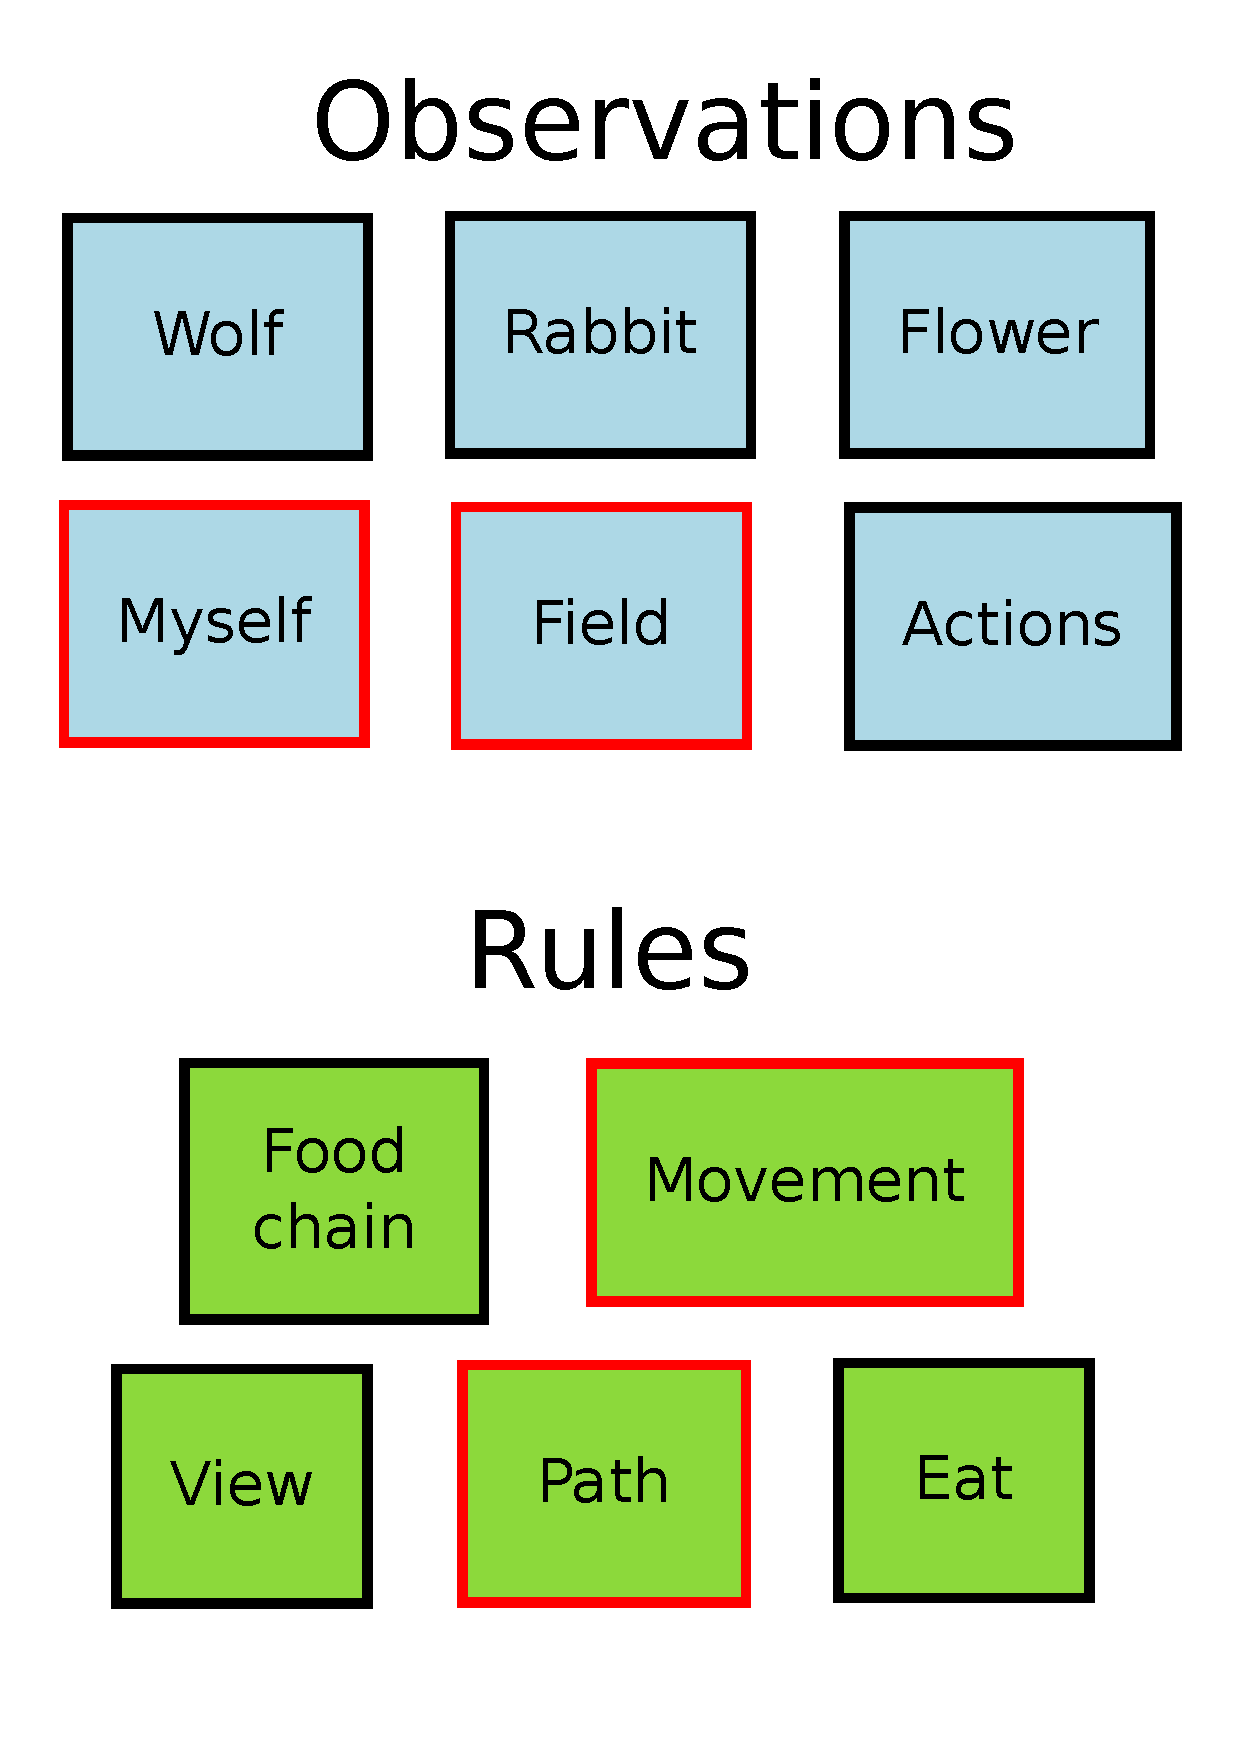
\includegraphics[keepaspectratio=true, scale=0.4]{module_combination.pdf}
		\caption
		{
			\label{module_combination}
			Knowledge base of a rabbit divided into observations modules (dot ones) and theory modules (plain ones).
		}
	\end{figure}

	We have presented different way to use agent knowledge via module combination.
	But these combinations are also a kind of knowledge and it can be known by the agent.
	For the agent it is meta-knowledge on his knowledge, more precisely in this case it is knowledge about the use of his knowledge.
	This meta-knowledge is a part of the common theory of an agent and could be represented by theory modules.
	But to clarify the design of agent knowledge we dedicated a new kind of modules to represent it: meta-knowledge module.
	We define two kind of this modules: combination module and decision module.
	
	\begin{definition}[Combination module]
		A combination module is meta-knowledge module which represent an ASP modules combination.	
		The purpose of these modules is to represent simple behaviours and factorise meta-knowledge.
	\end{definition}
	
	A module combination can represent agent behaviour and by using meta-knowledge modules we can represent it in a elegant way.
	Most simple behaviour can be represented by a simple list of modules to combine, like in examples \ref{hide_example}, 
	\ref{feed_example} and figures \ref{hide_figure}, \ref{feed_figure}.
	The module combination \{\emph{Myself}, \emph{Wolf}, \emph{Field}, \emph{Move}, \emph{Eat}, \emph{Action}\} 
	and \{\emph{Myself}, \emph{Rabbit}, \emph{Flower}, \emph{Field},  \emph{Move}, \emph{Eat}, \emph{Action}\} 
	can respectively represent the \textit{run away} and the \textit{feed} behaviour of a rabbit.
	This two combinations of modules can be represented by meta-knowledge modules, in this case theses modules have knowledge on theory and observations modules.
	
	\begin{example}
		\label{hide_example}
		A meta-knowledge module which describe the \emph{hide} behaviour of rabbit:\newline
		\begin{module}{Run away}{6cm}
			\textbf{use\_module}("Myself").\newline
			\textbf{use\_module}("Wolf").\newline
			\textbf{use\_module}("Field").\newline
			\textbf{use\_module}("Move").\newline
			\textbf{use\_module}("Eat").\newline
			\textbf{use\_module}("Action").
		\end{module}
	\end{example}
	
	\begin{figure}
		\centering
		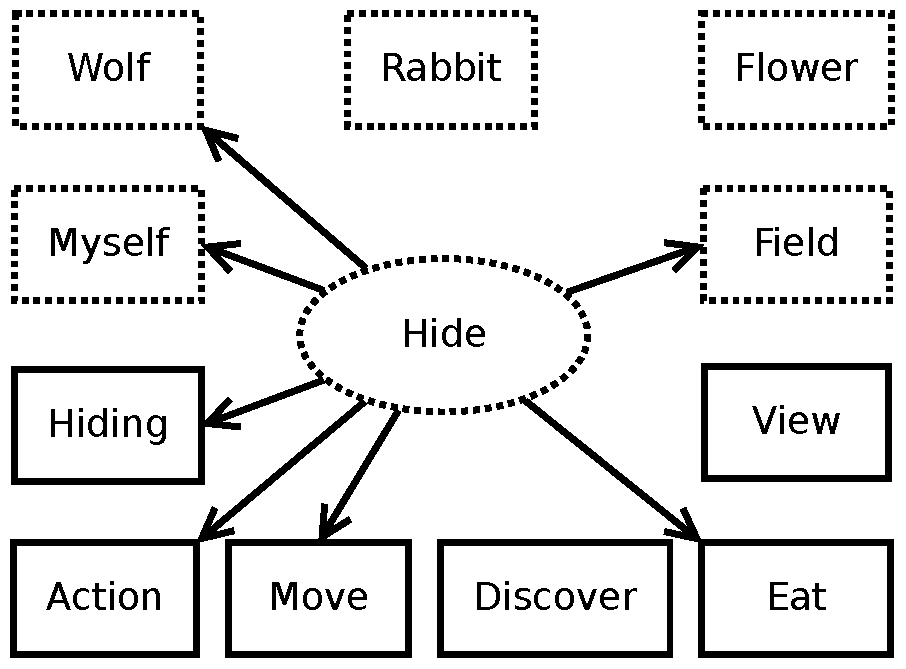
\includegraphics[keepaspectratio=true, scale=0.4]{hide.pdf}
		\caption
		{
			\label{hide_figure}
			A meta-knowledge module (circle one) about \textit{run away} behaviour linked to modules it combines.
		}
	\end{figure}
	
	\begin{example}
		\label{feed_example}
		A meta-knowledge module which describe the feed behaviour of rabbit:\newline
		\begin{module}{Feed}{6cm}
			\textbf{use\_module}("Myself").\newline
			\textbf{use\_module}("Rabbit").\newline
			\textbf{use\_module}("Flower").\newline
			\textbf{use\_module}("Field").\newline
			\textbf{use\_module}("Move").\newline
			\textbf{use\_module}("Eat").\newline
			\textbf{use\_module}("Action").
		\end{module}
	\end{example}
	
	\begin{figure}
		\centering
		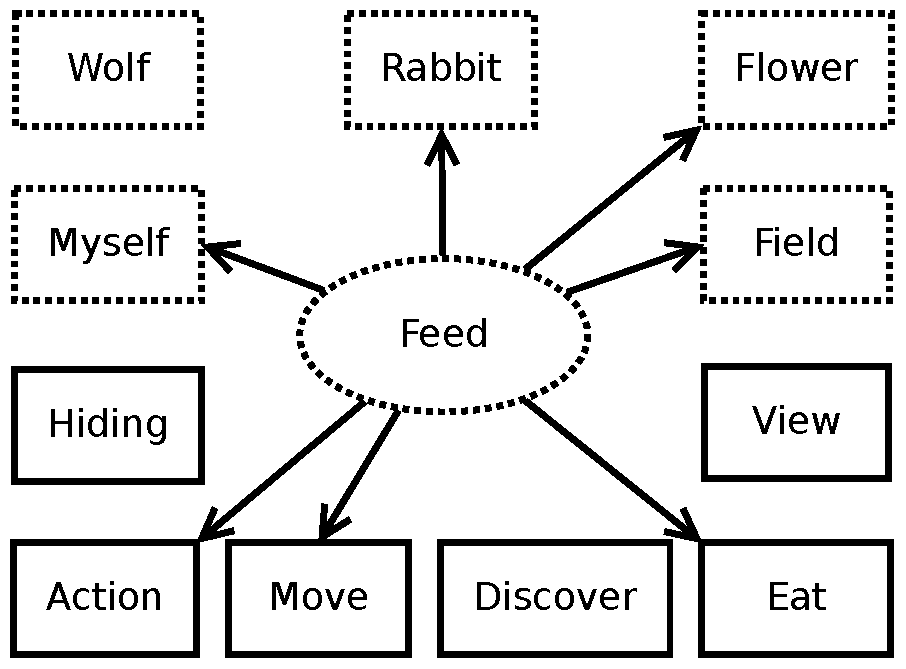
\includegraphics[keepaspectratio=true, scale=0.4]{feed.pdf}
		\caption
		{
			\label{feed_figure}
			A meta-knowledge module about \textit{feed} behaviour linked to modules it combines.
		}
	\end{figure}
	
	\begin{definition}[Decision module]
		A decision module is meta-knowledge module which define the conditions to use ASP modules combinations.	
		The purpose of these modules is to represent dynamic behaviours by performing decision on how to reason and use knowledge.
	\end{definition}
	
	To represent more complex behaviour we can have meta-knowledge modules which have knowledge on other meta-knowledge modules.
	For example we can represent the survive behaviour of a rabbit with such module, like in example \ref{survive_example} and figure \ref{survive_figure}.
	If a rabbit spotted a wolf it will use the \emph{Run away} module otherwise it will use the \emph{Feed} module.
	Regarding the situation the survive behaviour will be run way or approach flower.
	Meta-knowledge modules allows to represent such dynamic behaviours which are dependent of the evolution of the environment.
	Figure \ref{behaviour_tree} represent rabbit behaviour by a meta-knowledge module tree.
	The behaviour of a rabbit is survive, regarding the situation a rabbit is hunted by a wolf or not.
	When hunted, a rabbit have to run away or try to hide by go out of view range of his predator.
	If there is no predator he will explore his environment to find flower and when one is spotted go to eat it.
	
	\begin{example}
		\label{survive_example}
		A meta-knowledge module which describe the survive behaviour of a rabbit:\newline
		\begin{module}{Survive}{6.5cm}
			predator $\leftarrow$ position(wolf,Position).\newline
			\textbf{use\_module}("Hunted") $\leftarrow$ predator.\newline
			\textbf{use\_module}("Hunting") $\leftarrow$ not predator.
		\end{module}
	\end{example}
	
	\begin{figure}
		\centering
		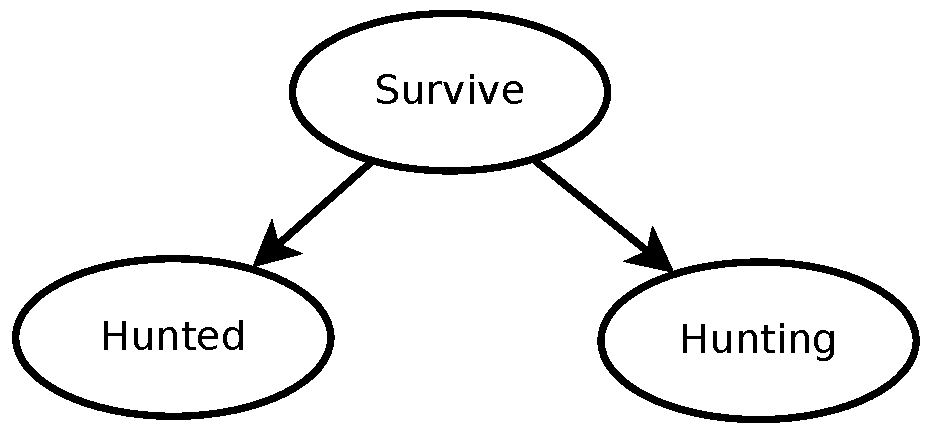
\includegraphics[keepaspectratio=true, scale=0.4]{survive.pdf}
		\caption
		{
			\label{survive_figure}
			A meta-knowledge module with knowledge about meta-knowledge module.
		}
	\end{figure}
	
	\begin{figure}
		\centering
		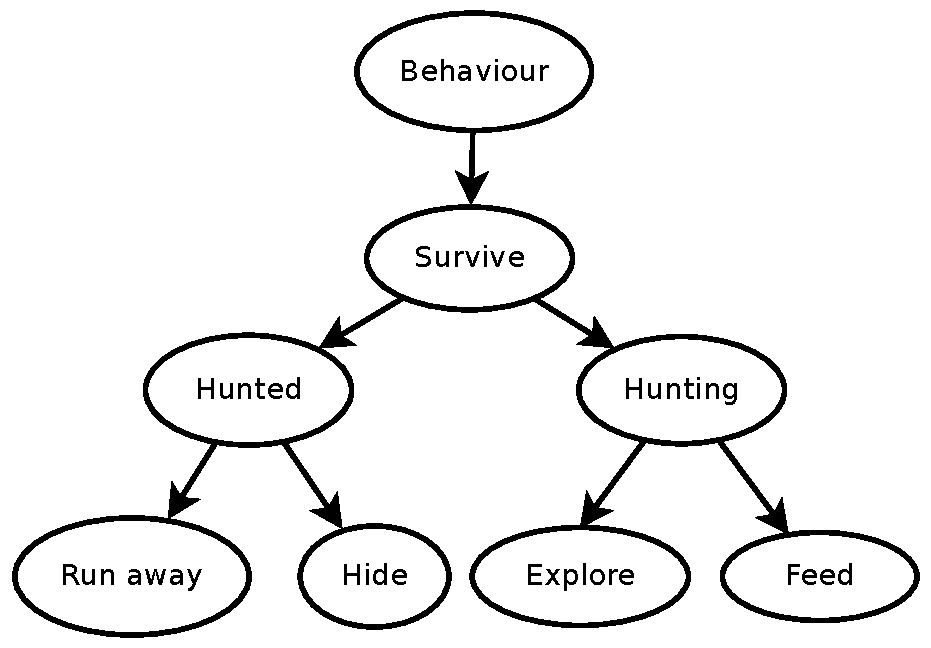
\includegraphics[keepaspectratio=true, scale=0.5]{behaviour_tree.pdf}
		\caption
		{
			\label{behaviour_tree}
			Representation of rabbit behaviour by a tree of meta-knowledge module.
			Decision module are represent by plain circle and combination modules by dot ones.
		}
	\end{figure}
	
\subsection{Architecture}

	The previous section shows that ASP modules can represent background knowledge, observations and behaviours of an agent.
	To use this representation we define a reasoning architecture and a framework to use it in agent application.
	As show in figure \ref{framework_figure}, we divide agent reasoning into three phase : acquisition, deduction, action.
	
	Reasoning cycle start when agent sensors retrieve new observations, it's the beginning of the acquisition phase.
	This phase deals with new observations and their consequences on old ones.
	New observations are stored in corresponding observations modules and old ones are update.
	If a wolf see a rabbit at position P at time step T, he will store the information \textit{position(rabbit,P)} in module \textit{Rabbit}.
	Now at T+1 the wolf see position P but no rabbit are at P, then the wolf have to remove the fact \textit{position(rabbit,P)} from module \textit{Rabbit}.
	During acquisition phase, agent memory is update to make it consistent with new observations.
	
	After acquire observations, an agent will reason on what he can do regarding the current state of the world: it is the deduction phase.
	The purpose of this reasoning phase is to deduce what actions are possible to perform.
	Here we use an agent reasoning architecture based on ASP modules where meta-knowledge modules are use for meta-reasoning.
	Meta-knowledge modules use agent observations to define his behaviour step by step.
	Knowledge produce by module combination is keep in next reasoning steps, 
	it means that answer set of the last reasoning step contains all deduction of previous ones.
	These last answer set contains action and their consequences on the environment and the agent.
	
	The figure \ref{modular_knowledge} represent rabbit knowledge by an ASP modules graph where a node is an ASP module, 
	undirected edge represent the use of a module and directed edge represent reasoning decisions.
	Here meta-knowledge module \textit{Movement} is used to represent a module combination which produce movement actions of a rabbit,
	other ones represent his behaviour like in figure \ref{behaviour_tree}.
	The reasoning phase will start by using \textit{Behaviour} module which just specify to use \textit{Survive} one.
	By combining \textit{Survive} module and wolf observation the rabbit will decide if he is hunted or have to hunt.
	If he is hunted he will then combine \textit{Hunted} with wolf observations to decide if run away or hide is the best solution,
	for example if the wolf is very near it is very risky to hide then run away will be choose.
	If there is no wolf the rabbit will use \textit{Hunting} with flower observation, if there is no flower he will use \textit{Explore} module
	and \textit{View} to try to find something to eat (\textit{View} module should contains some knowledge about view range).
	If there is flower in his observations, a rabbit will use \textit{Feed} to produce actions will allows him to approach and eat flowers.
	
	Now the agent have to choose which actions to perform, it means choose an answer set which allows him to approach or reach his goals.
	To make this choice we can use constraint or use some modules to compute score to rank answer set.
	For example module \textit{Eat} can compute the number of action a predator have to perform to eat a prey.
	Then this module can be use by a rabbit to rank movement action to go far away from a wolf or to approach and eat a flower.
	After choosing the best answer set, corresponding actions are performed and 
	the cycle continue by the acquisition of the real effect of theses actions on the environment.

	\begin{figure}
		\centering
		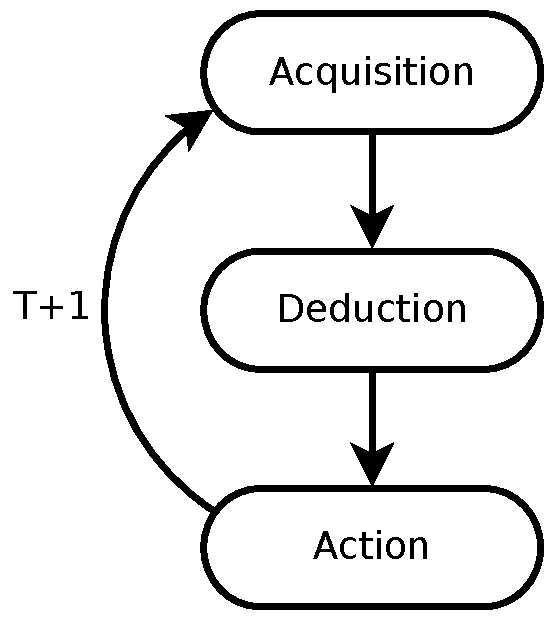
\includegraphics[keepaspectratio=true, scale=0.4]{framework.pdf}
		\caption
		{
			\label{framework_figure}
			Agent reasoning cycle.
		}
	\end{figure}

	\begin{figure}
		\centering
		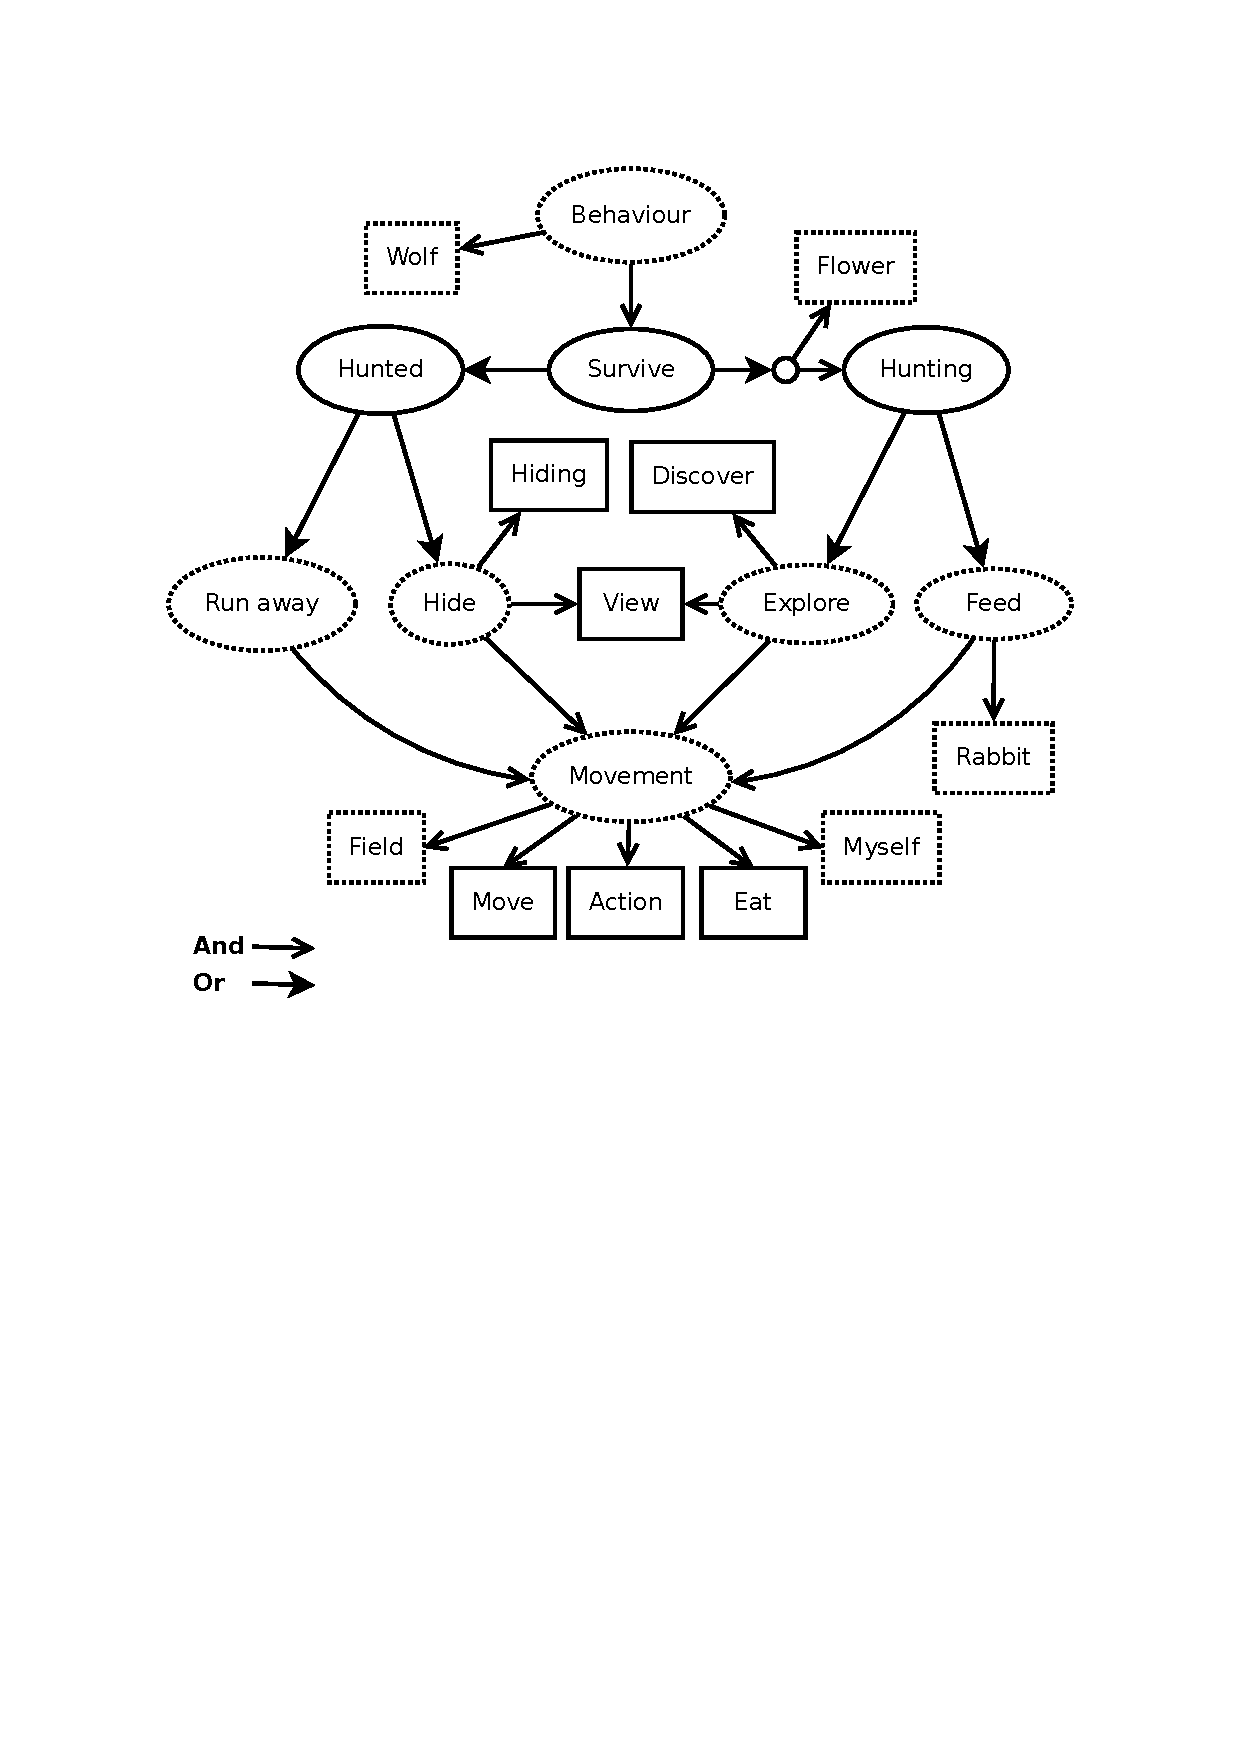
\includegraphics[keepaspectratio=true, scale=0.5]{modular_knowledge.pdf}
		\caption
		{
			\label{modular_knowledge}
			Representation of rabbit knowledge by an ASP modules graph.
		}
	\end{figure}
	
\subsection{Implementation}

	To allow an agent to use our method for reasoning in dynamic environment we implemented this framework.
	Algorithm \ref{framework_algorithm} represent a simplified version of this tool.
	
	Input is a set of modules and output is a set of answer set which contains actions that an agent can perform on its environment.
	It start by computing the combination of input modules and retrieve its answer sets by using the solver \emph{clingo}.
	Answer set are exploit in a deep first exploration by extracting keyword which define the combination of modules to use in the next reasoning step.
	When the answer set is totally parsed, we convert the current answer set into an ASP module and add it to the next combination of modules.
	Then, this combination is use for the next reasoning step and cycle continue.
	Finally, when there is no more module to combine it return a set of answer set.

	Let's take again the example of the figure \ref{modular_knowledge} and let's suppose that the rabbit just receive a set of new observation from its sensors.
	First our agent will combine theses new observations with the module \emph{Behaviour} to decide if he is hunted or have to hunt.
	Let's suppose that observations contains a wolf position, then the next combination of module to use is \{\emph{Hunted}\}.
	The wolf is too near to try to hide, so the next combination of module to use is \{\emph{Run away}\} which just specify to use \{\emph{Movement}\}.
	Finally this module will specify that the last combination of module to use is \{\emph{Myself}, \emph{Field}, \emph{Action}, \emph{Move}, \emph{Eat}\}.
	Then the algorithm will return all answer set of this combination, each answer will contain an movement action and its consequences, 
	for example the number of movement the wolf have to perform to catch the rabbit.
	
	In this example we can see that only a part of the knowledge is use for reasoning: 
	meta-knowledge modules \emph{Hide}, \emph{Hunting}, \emph{Explore} and \emph{Feed} are not used.
	Observations about flowers and knowledge about view are not used.
	The same knowledge can be represented in only one ASP program, but in this case all knowledge is use.
	Regarding this monolithic representation our method allows to reduce reasoning search space.
	
	Reasoning always finish when an agent use a module graph which is acyclic like in figure \ref{modular_knowledge}.
	To represent behaviours it is quite intuitive to make a tree of meta-knowledge modules, 
	where the root is the most abstract behaviour and deeper one are more specific.

	\begin{algorithm}
	\caption{Combine}
	\label{framework_algorithm}
	\begin{algorithmic}[1]
	\STATE INPUT : <M> M a set of ASP modules
	\STATE OUTPUT : AS a set of answer set
	\newline
	\STATE AS a set of answer set
	\newline
	\STATE AS $\leftarrow$ \textit{clingo}(M)
	\newline
	\FOR {each answer set S of AS}
		\STATE M $\leftarrow \emptyset$ 
		\newline
		\STATE // Extract keywords
		\FOR {every literal L of S}
			\IF {L = "use\_module(Module)"}
				\STATE M $\leftarrow$ M $\cup$ Module
				\STATE S $\leftarrow$ S $/$ L
			\ENDIF
		\ENDFOR
		\newline
		\IF {M $\neq$ $\emptyset$}
			\STATE // Add S to M as a module
			\STATE M $\leftarrow$ M $\cup$ module(S)
			\STATE combine(M)
		\ENDIF
	\ENDFOR
	\newline
	\RETURN AS
	\end{algorithmic}
	\end{algorithm}

\section{Experiments}

	To evaluate our work we implemented the algorithm \ref{framework_algorithm} and use it in a toy application based on the survival game example.
	In this application, the environment is a grid where agent are located on a square.
	Agents act turn by turn and have limited number of actions per turn.
	Theses actions can be: move to square or eat an agent.
	To eat his prey, a predator have to be on the same square.
	These experimental results focus on the reasoning time of a rabbit regarding a specific scenario.
	We compare modular and monolithic reasoning time: the first one needs multiple step to reach the module combination
	which correspond to the situation and the second one use directly the entire knowledge base (the background knowledge and all observations).
	In these experiments, the module combination \{\emph{Field}, \emph{Move}, \emph{Action}, \emph{Eat}, \emph{Myself}\} is always use at the end of reasoning.
	Difference between modular and monolithic representation is that the first one can avoid the use of flowers observation or hiding possibility.
	
\subsection{Context}
	
	In these experiments, the rabbit use the algorithm \ref{framework_algorithm} for reasoning.
	His observations concern the entire map, he knows what is on each square, it include the position of wolfs, flowers and hiding place.
	The figure \ref{modular_knowledge_experiment} represent the modular knowledge of the rabbit in these experiments.
	It is a simplified version where rabbit have two behaviours: \textit{run away} and \textit{feed}.
	Monolithic representation always use the entire knowledge base which correspond to the module combination
	\{\textit{Myself}, \textit{Wolf}, \textit{Flower}, \textit{Field}, \textit{Move}, \textit{Action} \textit{Eat}, \textit{Hiding}\}.
	
	\begin{figure}
		\centering
		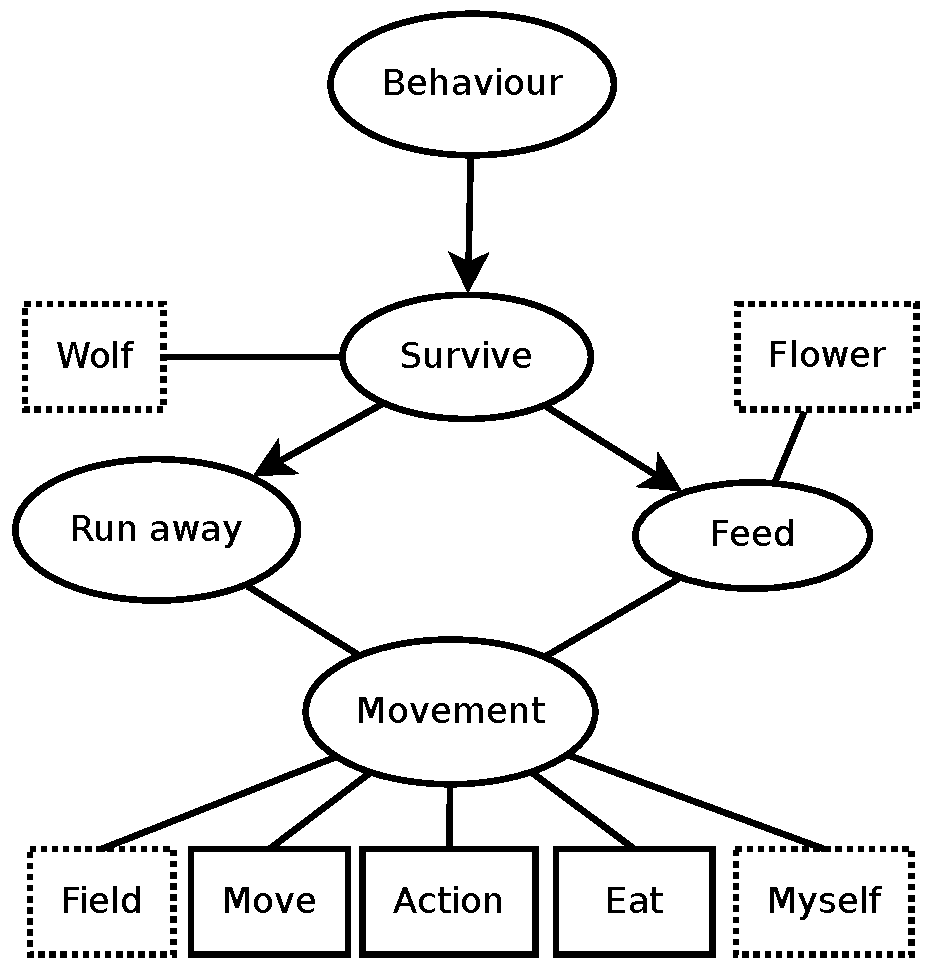
\includegraphics[keepaspectratio=true, scale=0.4]{modular_knowledge_experiment.pdf}
		\caption
		{
			\label{modular_knowledge_experiment}
			Rabbit knowledge in experiments, simplified to behaviours \emph{hide} and \emph{feed}.
		}
	\end{figure}
	
	For these experiment we use four different environment represented by figure \ref{environment_1}, \ref{environment_2} and \ref{environment_3}.
	The fourth one is equivalent to third one but ten time bigger in number of squares, flowers and hiding place.
	Our evaluation is based on height scenarios: for each environments, we evaluate rabbit reasoning time regarding if a a wolf is present or not.
	In scenarios where there is a wolf, reasoning about flower is useless because hiding have a bigger priority.
	When there is no wolf, reasoning about hiding is a loose of time because eating flower is more important.
	Here, we show that modular reasoning can be useful to optimize reasoning by avoiding a part of agent knowledge which is not necessary in the current situation.
	In all scenario, monolithic reasoning consider movement to hiding and eating possibilities regardless the presence of a wolf.
	Modular reasoning consider movement to hide when there is a wolf and consider eating when there is no predator.
	
	The figure \ref{environment_1} represent the first scenario where there is no flower and no hiding place.
	In this scenario the rabbit just consider the movement he can perform without being catch by his predator at the next turn.
	This scenario is used to evaluate the time we loose when modularity reasoning does not reduce search space.
	The figure \ref{environment_2} represent the second scenario where there is 4 flowers and 4 hiding places.
	In this scenario, when there is no wolf the time loose by multiple step of reasoning is just compensate by the reduction of search space.
	The figure \ref{environment_3} represent the third scenario, here our agents are in a field 25 flowers and 25 hiding place which are on the same square as flowers.
	Fourth scenario is a ten times bigger extension of the third one where the rabbit is in a field of 250 flowers and hiding place. 
	In these two last scenario, the number of flowers and hiding place is sufficient for modular representation to reduce reasoning time.
	
	\begin{figure}
		\centering
		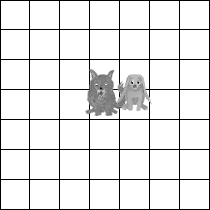
\includegraphics[keepaspectratio=true, scale=0.5]{environment_1.png}
		\caption
		{
			\label{environment_1}
			Environment 1, a rabbit and a wolf without flowers and no place to hide.
		}
	\end{figure}

	\begin{figure}
		\centering
		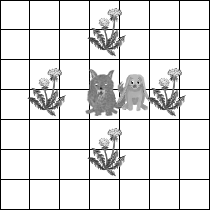
\includegraphics[keepaspectratio=true, scale=0.5]{environment_2.png}
		\caption
		{
			\label{environment_2}
			Environment 2, a rabbit, a wolf, 4 flowers and 4 hiding places (grass).
		}
	\end{figure}
	
	\begin{figure}
		\centering
		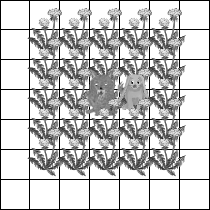
\includegraphics[keepaspectratio=true, scale=0.5]{environment_3.png}
		\caption
		{
			\label{environment_3}
			Environment 3, a rabbit and a wolf in a field of 25 flowers and 25 hiding places (same position as flower).
		}
	\end{figure}
	
\subsection{Results}

	\begin{table*}
		\label{experiment_results}
		\centering
		\begin{tabular}{ | c | c | c | c | c | c | c | c | }
		\hline
		Environment & Flower & Hiding place & Wolf & Representation & Time average & T-test & Runs\\	
		\hline
	 	\multirow{4}{*}{1} & \multirow{4}{*}{0} & \multirow{4}{*}{0} & \multirow{2}{*}{yes} & monolithic & 0.135 s & \multirow{2}{*}{0} & \multirow{16}{*}{1000} \\
		& & & & modular & 0.149 s & & \\ \cline{4-7}
		& & & \multirow{2}{*}{no} & monolithic & 0.107 s & \multirow{2}{*}{0} & \\
		& & & & modular & 0.119 s & & \\ \cline{1-7}
		\multirow{4}{*}{2} & \multirow{4}{*}{4} & \multirow{4}{*}{4} & \multirow{2}{*}{yes} & monolithic & 0.181 s & \multirow{2}{*}{0} & \\
		& & & & modular & \textbf{0.169 s} & & \\ \cline{4-7}
		& & & \multirow{2}{*}{no} & monolithic & 0.151 s & \multirow{2}{*}{$2.115E-5$} & \\
		& & & & modular & 0.152 s & & \\ \cline{1-7}
		\multirow{4}{*}{3} & \multirow{4}{*}{25} & \multirow{4}{*}{25} & \multirow{2}{*}{yes} & monolithic & 0.416 s & \multirow{2}{*}{0} & \\
		& & & & modular & \textbf{0.277 s} & & \\ \cline{4-7}
		& & & \multirow{2}{*}{no} & monolithic & 0.383 s & \multirow{2}{*}{0} & \\
		& & & & modular & \textbf{0.314 s} & & \\ \cline{1-7}
		\multirow{4}{*}{4} & \multirow{4}{*}{250} & \multirow{4}{*}{250} & \multirow{2}{*}{yes} & monolithic & 3.838 s & \multirow{2}{*}{0} & \\
		& & & & modular & \textbf{1.963 s} & & \\ \cline{4-7}
		& & &  \multirow{2}{*}{no} & monolithic & 3.819 s & \multirow{2}{*}{0} & \\
		& & & & modular & \textbf{2.739 s} & & \\ \cline{1-7}
		\hline
		\end{tabular}
		\caption
		{
			Experimental results of rabbit reasoning time on 8 scenarios of 4 different environments.
			For each method it shows reasoning time average of 1000 runs and T-test result.
		}
	\end{table*}

	These experiments focus on rabbit reasoning time regarding modular and monolithic representation on 8 scenarios.
	This time correspond of the run of algorithm \ref{framework_algorithm}, which include clingo solving and answer set parsing.
	The time we use is user one, to have a relevant value we compute the average running time on 1000 runs for each methods on each scenarios.
	These 16 sequences of 1000 runs test have been perform consequently in the same running conditions on a Intel Core 2 Duo P8400 2.26GHz CPU.
	Table \ref{Experiment_tab} resume these experimental results.
	
	In scenario 1, figure \ref{environment_1}, when there is a wolf, monolithic reasoning run is about 0.135 and modular one is about 0.139.
	When there is no wolf monolithic reasoning run is about 0.107 and modular one is about 0.119.
	Here use of multiple reasoning step by modular representation cause more time for reasoning because it does not reduce search space.
	In scenario 2, figure \ref{environment_2}, in the case of the presence of a wolf, 
	run time of monolithic reasoning up to 0.181 because it now consider 4 flowers and 4 hiding places,
	and modular reasoning time just up to 0.169 because it does not consider flowers.
	If there is no wolf, monolithic and modular reasoning time is almost the same.
	The time loose by reasoning about hiding in monolithic representation is the same as the time loose by multiple step reasoning.
	In these environment modular reasoning is a little bit more efficient than monolithic one.
	For scenario 3, figure \ref{environment_3}, modular reasoning is more efficient in both case.
	The proportion of flowers and hiding place is sufficient to make search space reduction interesting.
	When reasoning about hiding is the priority, modular reasoning take 30\% less time than monolithic one and
	18\% less time when reasoning about eating is the most important.
	As the number observation increase, modular representation become more interesting, in scenario 4 when there is a wolf it take 49\% less time to
	compute hiding actions and 32\% less time for reasoning about rating.
	
	These experiment show that modular knowledge representation and knowledge about module combination can be useful to reduce reasoning search space.
	Here we show that this representation can be always more efficient than monolithic one when the entire knowledge base is not necessary to solve every situation.
	Designing such reasoning pattern imply to find the balance between the time loose by multiple reasoning step and search space reduction.
	
\section{Conclusions and Outlook}

	We provide a method based on ASP modules to design agent knowledge and reasoning.
	This representation allows to intuitively implements dynamic behaviours via meta-reasoning.
	We also provide a framework which allows agent reasoning by module combination.
	Regarding an equivalent monolithic representation, a first improvement of our method is the reduction of reasoning search space.
	Its also cause reduction of code size because modules are reusable for multiple purposes.
	
	In this paper, agent reasoning is very directed by meta-knowledge modules, 
	an interesting outlook will be to give the possibility to the agent to really choose which module combination he want to use.
	Make agent able to construct themselves a reasoning architecture like the one of figure \ref{modular_knowledge} is also an interesting research topic.
	Learning can also concern module content, an agent could choose to create new observations modules for storing specific information.
	Modular representation give new perspective for meta-reasoning and learning.
%
% The following two commands are all you need in the
% initial runs of your .tex file to
% produce the bibliography for the citations in your paper.
\bibliographystyle{abbrv}
\bibliography{ASP_Modules}  % sigproc.bib is the name of the Bibliography in this case
% You must have a proper ".bib" file
%  and remember to run:
% latex bibtex latex latex
% to resolve all references
%
% ACM needs 'a single self-contained file'!
%

%\nocite{*}

\end{document}
